\documentclass[10pt,letter]{report}
\usepackage{import}
\import{../../../../sistema/}{rutas}
\usepackage[T1]{fontenc}
%\usepackage[letterpaper, headsep=60pt, headheight=2cm]{geometry}
\usepackage{verbatim}
\usepackage[utf8x]{inputenc}
\usepackage[table]{xcolor}
\usepackage{float}
\usepackage{import}
\usepackage{textcomp}
\usepackage{ifthen}
%\usepackage[spanish,mexico-com]{babel}
\usepackage{pdflscape}
\usepackage{mathrsfs}
\usepackage{amsmath}
\usepackage{amssymb}
\usepackage{bbm}
\usepackage{tikz}
\usepackage{fp}
\usepackage[autolanguage]{numprint}
\usepackage{array}
\usetikzlibrary{shapes}
\usepackage{subfigure}
\usepackage{ucs}
\usepackage[utf8x]{inputenc}
\usepackage{fontenc}
\usepackage{graphicx}
\usepackage{anysize}
\usepackage{relsize}
\usepackage{booktabs}

\usepackage{fancyhdr}
\usepackage[all]{xy}
\setlength{\headheight}{13.1pt}
\makeatletter\renewcommand\theenumi{\@alph\c@enumi}\makeatother
\renewcommand\labelenumi{\theenumi)}
\usepackage{amsthm}
\usepackage{enumerate}

\usepackage[]{mdframed}

\usepackage{marvosym}
\usepackage{tikzsymbols}
\usepackage{imakeidx}%for indexes
%\usepackage{tocbibind}
\usepackage{background}
\usepackage{titlesec}
\usepackage{multirow}
\usepackage{etoolbox}
\usepackage{fmtcount}
\usepackage{datetime}
\usepackage[bookmarks=true]{hyperref}%must be at the end of preamble
\usepackage[toc,section=subsection, acronym, shortcuts]{glossaries}
\usepackage[open,openlevel=0]{bookmark}
\usepackage{lipsum}
\usepackage{multicol}
\usepackage{wrapfig}
\usepackage[titletoc]{appendix}
\usepackage{sectsty}

\usepackage{titlesec}
\usepackage{pdfpages}
%---------------Formato Numeros \numprint-------------
\npdecimalsign{.}
\nprounddigits{2}
\npthousandsep{,}

%-----------------Espacio en blanco--------------------
\newcommand{\espacio}[1]{\vspace{#1}\begin{center}\textit{[BLANK SPACE]}\end{center}\newpage}
\newcommand{\inserta}{\colorbox{principal}{\textcolor{orange}{Insertar}}}
\input{disenno}

%----------------------------Generales----------------------------
\newcommand{\tipoAvaluo}{Equity Capital}
\newcommand{\bienesValuados}{capital accionario de la sociedad \empresaSolicitante}%nombre del bien que se va a valuar
\newcommand{\lugarInforme}{the State of Mexico}

%--------------------Fechas---------------------------
\newcommand{\diainforme}{25} %dia del informe
\newcommand{\mesinforme}{3} %mes del informe
\newcommand{\annoinforme}{2024} %año del informe

\newcommand{\diavalores}{31} %dia de valores
\newcommand{\mesvalores}{12} %mes de valores
\newcommand{\annovalores}{2023} %año de valores

\newcommand{\diainspeccion}{1} %dia de inspeccion
\newcommand{\mesinspeccion}{1} %mes de inspeccion
\newcommand{\annoinspeccion}{2022} %año de inspeccion

\newcommand{\fechaInforme}{\monthname[\mesinforme]{} \diainforme{}, \annoinforme}
\newcommand{\fechaValores}{\monthname[\mesvalores]{} \diavalores{}, \annovalores}
\newcommand{\fechaValoresCorto}{\mesvalores/\diavalores/\annovalores}
\newcommand{\fechaInspeccion}{\monthname[\mesinspeccion]{} \diainspeccion{}, \annoinspeccion}

%----------------------------Perito Valuador---------------------
\newcommand{\peritoValuador}{DiegoPerezcano_cp2}
\import{\rutaValuatex/documentos_modelo/peritos/peritos/}{\peritoValuador}

%------------------------Perito Auxiliar-------------------
\newcommand{\peritoAuxiliar}{n/a}
\ifthenelse{\equal{\peritoAuxiliar}{n/a}}{ }{\import{\rutaValuatex/documentos_modelo/peritos/auxiliares/}{\peritoAuxiliar}}

%--------------Datos del solicitante-------------
\newcommand{\empresaSolicitante}{VIVO TECH, S.A. de C.V.}
\newcommand{\empresaCorto}{VIVO TECH}
\newcommand{\rfcEmpresa}{VTE210820IM1}
\newcommand{\personaSolicitante}{Cal Li}
\newcommand{\caracterSolicitante}{Sole Administrator}

%--------------Datos del propietario-------------
\newcommand{\nombrePropietario}{\inserta}

%-------------Vigencia----------------------------
\newcommand{\vigenciaInforme}{1(One) year}
\newcommand{\notaVigencia}{si}


%---------------Ubicacion del bien sujeto de valuaci\'on
\newcommand{\descripcionBien}{Equity Capital of \empresaSolicitante}%en que consiste el bien que se va a valuar.
\newcommand{\ubicacionBien}{Mexico City}
\newcommand{\rfcBien}{\inserta}

%------------Uso de la valuación---------------
\newcommand{\usoAvaluo}{financial and tax purposes}
%--------------Desarrollo del avalúo en la especie-------------------
\newcommand{\EFde}{2021}
\newcommand{\EFhasta}{2023}
\newcommand{\EFdeHasta}{2021 to 2023}

%----------------Parámetros Peers--------------------------
%__________Multiplo________________
\newcommand{\peersa}{Enterprise Value to Sales}
\newcommand{\peersb}{Enterprise Value to EBIT}
\newcommand{\peersc}{Ratio of Firm Value to EBITDA}
\newcommand{\peersd}{Ratio of Offer Price to Book Value}
\newcommand{\peerse}{Ratio of Offer Price to Book Value}

%____________x veces________
\newcommand{\peersaTo}{Ventas}
\newcommand{\peersbTo}{EBIT}
\newcommand{\peerscTo}{EBITDA}
\newcommand{\peersdTo}{Valor en libros}
\newcommand{\peerseTo}{Valor en libros}

%___________Valor Múltiplo____________
\newcommand{\peersaMult}{0.9518}
\newcommand{\peersbMult}{9.2371}
\newcommand{\peerscMult}{6.24}
\newcommand{\peersdMult}{1.52}
\newcommand{\peerseMult}{1.52}

%___________Estadístico____________

\newcommand{\peersaEst}{Mediana}
\newcommand{\peersbEst}{Mediana}
\newcommand{\peerscEst}{Mediana}
\newcommand{\peersdEst}{Mediana}
\newcommand{\peerseEst}{Mediana}

%============ WACC ===============
%---------------------- RF ------------------------------
\newcommand{\rfBase}{bono mexicano a 10 años}
\newcommand{\rfValor}{9.10}

%---------------------- Beta ----------------------------
\newcommand{\valorBeta}{1.29}
\newcommand{\betaDesapalancada}{1.0568}
\newcommand{\betaReapalancada}{1.5149}
%-----------------------Premio de Mercado (ERP)----------------------------
\newcommand{\mercadoAccionario}{mexicano}%mexicano o americano
\newcommand{\erpValor}{3.50}

%----------------------Prima de tamaño-----------------
\newcommand{\sizePrime}{5.01}

%-----------------------Costo de Capital (ke)--------------------
\newcommand{\keValor}{18.60}

%----------------------Costo de deuda (Kd)-----------------------
\newcommand{\kdValor}{0}

%----------------------- Valor Wacc----------------------------
\newcommand{\waccValor}{18.60}

%=============== DCF ======================
\newcommand{\periodoProyeccion}{2024 a 2028}
\newcommand{\proyCagr}{18.12}
\newcommand{\proyEbitMargin}{7.15}

\newcommand{\tasaFiscal}{30.00}
\newcommand{\reinvestmentRate}{46.70}


%============== RFR (Relief from royalties)==========
\newcommand{\tasaRegalias}{2.00}
\newcommand{\estadisticoTasaRegalias}{Percentil 25}


%============== CIFRAS ======================
\newcommand{\valorDCF}{12,895,851}
\newcommand{\valorDCFLetra}{Doce millones ochocientos noventa y cinco mil ochocientos cincuenta y uno} 

\newcommand{\valorPEERS}{0}
\newcommand{\valorPEERSLetra}{cero} 

\newcommand{\valorFirma}{19,863,282}
\newcommand{\valorFirmaLetra}{Nineteen million eight hundred sixty-three thousand two hundred eighty-two} 

\newcommand{\valorCapital}{16,409,631}
\newcommand{\valorCapitalLetra}{Sixteen million four hundred nine thousand six hundred thirty-one} 

\newcommand{\valorRFR}{0}
\newcommand{\valorRFRLetra}{cero} 

\newcommand{\valorResidual}{0}
\newcommand{\valorResidualLetra}{cero} 

\newcommand{\valorActivoIntangible}{0}
\newcommand{\valorActivoIntangibleLetra}{cero} 

\newcommand{\valorCapitalIntangible}{0}
\newcommand{\valorCApitalIntangibleLetra}{cero} 

\newcommand{\moneda}{pesos}
\newcommand{\monedaCode}{MXN}









%\makenoidxglossaries

%\import{\rutaValuatex/documentos_modelo/}{glosario}
%\import{\rutaValuatex/documentos_modelo/}{acronimos}
\newglossaryentry{beta}
{
        name=Beta ($\beta$),
        plural=Betas,
        description={El coeficiente Beta ($\beta$) es una medida de volatilidad que estima el riesgo sistem\'atico de un activo}
}

\newglossaryentry{cashNeq}
{
        name=Cash \& Eq,
        description={Efectivo y equivalentes}
}

\newglossaryentry{efectivetaxrate}
{
        name=Effective Tax Rate,
        description={Tasa fiscal efectiva}
}

\newglossaryentry{enterprisevalue}
{
        name=Enterprise value,
        description={Valor de la empresa}
}

\newglossaryentry{equityvalue}
{
        name=Equity value,
        description={Valor del capital accionario}
}

\newglossaryentry{exitmultiple}
{
        name=Exit multiple,
        description={M\'ultiplo de salida}
}

\newglossaryentry{expdebt}
{
        name=Explicit Debt,
        description={Deuda expl\'icita}
}

\newglossaryentry{fairvalue}
{
        name=Fair Value,
        description={Valor razonable o valor justo de mercado}
}

\newglossaryentry{firmvalue}
{
        name=Firm Value,
        description={Valor de la firma o empresa}
}

\newglossaryentry{growthrate}
{
        name=Growth Rate,
        description={Tasa de crecimiento de ingresos netos}
}

\newglossaryentry{incomestatement}
{
        name=Income Statement,
        description={Estado de Resultados}
}

\newglossaryentry{investmentcapital}
{
        name=Investment Capital,
        description={Capital Invertido (IC)}
}

\newglossaryentry{leveredbeta}
{
        name=beta apalancada,
        plural=betas apalancadas,
        description={Levered beta}
}

\newglossaryentry{marketaproach}
{
        name=Market approach,
        description={Enfoque de mercado}
}

\newglossaryentry{netdebt}
{
        name=Net Debt,
        description={Deuda neta}
}

\newglossaryentry{nopat}
{
        name=NOPAT,
        description={Flujo de Operaci\'on Neto}
}

\newglossaryentry{projectvaluation}
{
        name=Project Valuation,
        description={Valor razonable del proyecto de inversi\'on}
}

\newglossaryentry{riskfreerate}
{
        name=Risk Free Rate,
        description={Tasa Libre de Riesgo}
}

\newglossaryentry{sizeprime}
{
        name=Size Prime,
        description={Prima por tama\~no}
}

\newglossaryentry{terminalvalue}
{
        name=Terminal Value,
        description={Valor terminal}
}

\newglossaryentry{totaldebt}
{
        name=Total Debt,
        description={Deuda total}
}

\newglossaryentry{valuedrivers}
{
        name=Value drivers,
        description={Elevadores de Valor}
}
\newacronym{cagr}{CAGR}{Tasa compuesta de crecimiento anual}
\newacronym{capm}{CAPM}{CAPITAL ASSET PRICING MODEL}
\newacronym{chic}{CHIC}{Sociedades de Inversi\'on Cerradas}
\newacronym{crp}{CRP}{Riesgo Pa\'is}

\newacronym{dcf}{DCF}{Flujo de efectivo descontado (Discounted Cash FLow)}
\newacronym{erp}{ERP}{Premio de Mercado}
\newacronym{etr}{ETR}{Tasa Fiscal Efectiva}
\newacronym{fcff}{FCFF}{Flujo de efectivo libre a la Firma (Free Cash Flow to Firm)}
\newacronym{fcfe}{FCFE}{Flujo de efectivo libre al Capital (Free Cash Flow to Equity)}
\newacronym{g}{G}{Tasa de Crecimiento de ingresos netos (Grow Rate)}
\newacronym{ke}{Ke}{Costo de Capital Accionario}
\newacronym{kd}{Kd}{Costo de la deuda}
\newacronym{kpi}{KPI}{Indicador clave de desempe\~no o indicadores de gesti\'on \textit{(Key Performance Indicator)}}
\newacronym{mpeem}{MPEEM}{Multi-Period Excess Earnings Method}
\newacronym{nav}{NAV}{Valor neto de activos}
\newacronym{nca}{NCA}{Activo No Corriente}
\newacronym{nwc}{NWC}{Capital de Trabajo Neto}
\newacronym{peers}{PEERS}{M\'ultiplos de Cotizaci\'on}
\newacronym{rfr}{RFR}{M\'etodo de Flujo de Ahorro en Regalias}
\newacronym{wacc}{WACC}{Weighted Average Costo of Capital}
\newacronym{wara}{WARA}{Weighted Average Return on Assets}

\usepackage{pdfpages}

\renewcommand{\espacio}[1]{\vspace{#1}\begin{center}\textit{[BLANK SPACE]}\end{center}\newpage}

\begin{document}

% Renombrar sección a inciso
\def\sectionautorefname{section}
\def\subsectionautorefname{section}
\def\subsubsectionautorefname{section}


\thispagestyle{plain}
\NoBgThispage
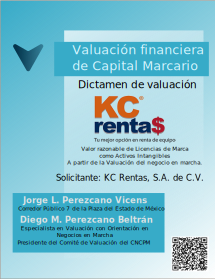
\includepdf[pages=-]{../0.portadas_eng/portada}

%-------------------------Índice-------------------------------
\newpage
\setcounter{page}{1}
\thispagestyle{fancy}
\tableofcontents

\newpage


\chapter{BACKGROUND.}\label{cap:1}
\thispagestyle{fancy}
%--------------------Datos del Valuador------------------
\section{EXPERT APPRAISER INFORMATION}\label{sec:a}

In \lugarInforme, on the \numberstringnum{\diainforme} day of the month of \monthname[\mesinforme] in the year \numberstringnum{\annoinforme}, I, \textbf{\textcolor{principal}{Diego Miguel Perezcano Beltrán, Public Broker No. 2 of the State of Mexico, a specialist in business valuation, holding a professional license from the Ministry of Public Education with the number 10548258}}; in my capacity as an EXPERT APPRAISER granted by the law; based on my technical knowledge and the application of valuation techniques, as provided for by Article 6, Section II, and other relevant provisions of the Federal Public Brokerage Law; Article 6, second paragraph, and Article 56 Bis of the Regulations of the Federal Public Brokerage Law; I hereby issue the following Equity appraisal report.
%------------------Datos del solicitante-----------------
\section{APPLICANT INFORMATION}\label{sec:b}
La sociedad \textcolor{principal}{\empresaSolicitante}, en lo sucesivo \textcolor{principal}{``\empresaCorto''}, por conducto del \textcolor{principal}{\personaSolicitante} en su car\'acter de \textcolor{principal}{\caracterSolicitante.}

\espacio{3cm}

\chapter{DATA OF THE ASSET SUBJECT TO VALUATION}\label{cap:2}
\thispagestyle{fancy}
\setcounter{section}{2}
%-----------------Datos del Propietario----------------
\section{OWNER'S INFORMATION}\label{sec:c}
The applicant presented me with the corporate documentation of \textcolor{principal}{\empresaSolicitante} (hereinafter \textcolor{principal}{``\empresaCorto''}), which is attached to this report as \textcolor{secundario}{APPENDIX 1}.
%-----------------Tipo de servicio de valuación------
\section{TYPE OF VALUATION SERVICE}\label{sec:d}
A petici\'on del solicitante se llev\'o a cabo un avalúo de \textcolor{principal}{\tipoAvaluo}.

%-----------------Vigencia-----------------------------
\section{REPORT VALIDITY}\label{sec:e}



The validity of this report is  \textcolor{terciario}{\vigenciaInforme{}} \footnote{In the absence of specific provisions regarding the validity of this type of valuation report, the one-year term mentioned in Article 3 of the Regulation of the Federal Fiscal Code was used.}.\\[5pt]


\textcolor{secundario}{Extrinsic or administrative validity:} The validity of an appraisal is determined by its purpose or intended use and depends on the time frame established, if applicable, by the competent authority or administrative institution utilizing the report.\\[10pt]


\noindent\textcolor{secundario}{Intrinsic validity:} A report will remain valid as long as there are no substantial changes in the fundamental conditions and premises that supported the calculation (\textit{ceteris paribus}). Any substantial changes could potentially affect the reliability of the conclusive figures of the valuation.\\


%---------------Descripción de los bienes Sujetos de valuación-----------
\section{DESCRIPTION OF THE VALUATION SUBJECT}\label{sec:f}
\begin{enumerate}[\thesection.1.]
\item El solicitante le proporcion\'o al valuador el t\'itulo de registro de la marca registrada \textcolor{principal}{\marca{}} la cual es explotada y/o tiene relaci\'on con los flujos de ingresos de la sociedad \textcolor{principal}{\empresaSolicitante}; misma que se detalla y se agrega al \textcolor{terciario}{AP\'ENDICE 1:}

\begin{figure}[H]
\centering
\includegraphics[width=.7\textwidth]{../0.imagenes/bien_1}\\
\end{figure}

\end{enumerate}

\textit{\underline{Nota 1}: El presente dictamen no consiste en una auditor\'ia de propiedad intelectual respecto de los derechos mencionados anteriormente, ni se puede considerar como un due diligence de propiedad intelectual de la marca mencionada por el solicitante; por lo que se asume como informaci\'on precisa y de buena fe, seg\'un se relaciona en la semblanza de la empresa que se agrega a este informe como \textcolor{terciario}{AP\'ENDICE 2.}}\\

\textit{\underline{Nota 2}: El valuador y su perito auxiliar no asumen responsabilidad alguna respecto de errores o imprecisiones en la informaci\'on mencionada en este inciso y su relaci\'on con los ingresos de la empresa sujeta de valuaci\'on que explota los beneficios de dichos activos intangibles; seg\'un se aprecia en sus estados financieros.}

%-----------------Ubicación del bien sujeto de valuavión
\section{LOCATION OF THE VALUATION SUBJECT}\label{sec:g}
La sociedad \textcolor{principal}{\empresaCorto}, con RFC \textcolor{peincipal}{\rfcEmpresa}, tiene su domicilio fiscal ubicado en \textcolor{principal}{\ubicacionBien.}
%-----------------Propósito----------------------
\section{VALUATION PURPOSE}\label{sec:h}
Estimar el Valor Razonable (\textit{\gls{fairvalue}}) del portafolio de activos intangibles mencionado en el  \autoref{sec:f}, con fecha de valores a \textcolor{principal}{\fechaValores}.
%------------------Uso de la valuación---------------
\section{VALUATION USE}\label{sec:i}


The applicant has informed the Appraiser that they require this report for \textcolor{principal}{\usoAvaluo}.



\newpage

\chapter{LEGAL BASIS AND PRELIMINARY CONSIDERATIONS.}\label{cap:3}
\thispagestyle{fancy}
\setcounter{section}{9}

\section*{LEGAL BASIS.}\label{sec:juridico}
The present analysis, as well as the opinions and conclusions of the undersigned appraiser, were developed in accordance with Article 6, Section II of the Federal Public Brokerage Law (LFCP), Article 56 bis of its regulations, international valuation standards, and the theoretical framework of corporate finance.\\

The following are various legal bases in Mexican regulations related to valuation reports:\\


\textcolor{principal}{Código de Comercio:}\\[10pt]

\textit{``Artículo 1252.- Los peritos deben tener título en la ciencia, arte, técnica, oficio o industria a que pertenezca la cuestión sobre la que ha de oírse su parecer, si la ciencia, arte, técnica, oficio o industria requieren título para su ejercicio.}\\[10pt]

\textit{Si no lo requirieran o requiriéndolo, no hubiere peritos en el lugar, podrán ser nombradas cualesquiera personas entendidas a satisfacción del juez, aun cuando no tengan título.}\\

\textit{La prueba pericial sólo será admisible cuando se requieran conocimientos especiales de la ciencia, arte, técnica, oficio o industria de que se trate, más no en lo relativo a conocimientos generales que la ley presupone como necesarios en los jueces, por lo que se desecharán de oficio aquellas periciales que se ofrezcan por las partes para ese tipo de conocimientos, o que se encuentren acreditadas en autos con otras pruebas, o tan sólo se refieran a simples operaciones aritméticas o similares.} \\[10pt] 

\textit{El título de habilitación de corredor público acredita para todos los efectos la calidad de perito valuador.''} (...)\\[10pt]

\textit{``Artículo 1257.- Los jueces podrán designar peritos de entre aquéllos autorizados como auxiliares de la administración de justicia por la autoridad local respectiva, o a solicitar que el perito sea propuesto por colegios, asociaciones o barras de profesionales, artísticas, técnicas o científicas o de las instituciones de educación superior públicas o privadas, o las cámaras de industria, comercio, o confederaciones de cámaras a la que corresponda al objeto del peritaje.  (...)''}\\[10pt]

\textit{``Artículo 1300.- Los avalúos harán prueba plena.}\\[10pt]


\textcolor{principal}{FEDERAL PUBLIC BROKERAGE LAW}\\[10pt]

\textit{``ARTICLE 6.- The public broker shall have the following responsibilities: (...)}\\[10pt]

\textit{II.- To act as an expert appraiser to estimate, quantify, and assess the goods, services, rights, and obligations submitted for consideration, whether by private appointment or by mandate of competent authority; (...)}\\[10pt]

\textit{VIII. Any other functions assigned to them by this and other laws or regulations.}\\[10pt]


\textit{The above-mentioned functions shall be understood without prejudice to the provisions of other laws and are not considered exclusive to public brokers.''}\\[10pt]



\textcolor{principal}{FEDERAL PUBLIC BROKERAGE LAW REGULATION}\\


``\textcolor{secundario}{ARTICLE 56 Bis.-} \textit{The public broker, in the exercise of their functions as an expert appraiser, may estimate, quantify, and assess the goods, services, rights, and obligations submitted for consideration by private appointment or by mandate of competent authority.}\\


\textit{The valuation report must be clear and objective, presenting the reasoning and sufficient information used to determine the conclusive value of the asset, service, right, or obligation. It must contain, at a minimum, the following indicative items:}

\begin{enumerate}[a)]

\item  Full name, number, and location of the Public Broker, along with their signature and seal; 
\item Applicant's information;
\item  Owner's information, including, if applicable, the basis for the information; 
\item  Type of valuation service;
\item Valuation validity, which is a mandatory requirement when there is a legal provision to that effect;
 \item  Description of the asset, right, service, or obligation subject to valuation;
 \item  When applicable, the location of the asset subject to valuation;
 \item  Purpose of the valuation report;
\item  Use of the valuation report;
\item  Preliminary considerations for valuation;
\item  Description of the valuation approaches applied;
\item  Inspection date;
\item  If applicable, the reference date for value;
\item  Valuation report date;
\item  Sources of information;
\item  Preliminary considerations before the conclusion; 
\item  Value conclusion;
\item  Photographic documentation, and 
\item  If applicable, annexes.

\end{enumerate}

\textit{Any observations regarding approaches, sources of information, elements, general limitations, among others, that affect the value conclusion, must be mentioned in the report.}\\

\textit{In cases where, due to the valuation service, territory, purpose, use, or the subject matter of the report requested from the public broker, it is evident that, based on specific regulations issued by a competent authority that are mandatory, the broker must issue or prepare the report using specific laws, standards, guidelines, manuals, or rules, the broker may choose to adhere solely to that regulation.}\\

\textit{In the case of auctions, valuations for judicial or administrative proceedings, or valuations requested by authorities where it is physically or materially impossible to conduct a physical inspection of the asset subject to valuation or obtain the corresponding documentation from the applicant or owner, it must be expressly stated in the report. The valuation will then be performed with the data and information available to the broker at the time and with the means at their disposal.''}\\




\textcolor{principal}{AGREEMENT ESTABLISHING GUIDELINES FOR PUBLIC BROKERS TO ISSUE APPRAISALS ISSUED BY THE SECRETARY OF COMMERCE AND INDUSTRIAL PROMOTION, PUBLISHED IN THE OFFICIAL GAZETTE ON MARCH 9, 1999.}\\[10pt]



\textit{``Article 2.- The valuation report issued by the public broker shall be composed of the following sections:}

\begin{enumerate}[I.]

\item Background;
\item Data of the asset or service subject to valuation; 
\item Legal basis and preliminary considerations; 
\item  Methodology employed;
\item  Development of the appraisal, and
\item  Conclusions.

\end{enumerate}

\textit{Furthermore, in all cases, the public broker must have complete documentary support regarding the market study conducted for the purposes of the appraisal. (...)}\\[10pt]

\textit{Article 12.- In valuations performed by public brokers for intangible assets, considering their nature or type, their values may be determined as follows:}

\begin{enumerate}[I.-]
\item By researching the market for similar or substitute goods and products based on commercial references, implied and calculated values, considering sales volumes and profitability, possible purchase and sale cases, or alternatively, royalty payments for the use and exploitation of patents, trademarks, or franchises;

\item In the case of projects, an analysis will be conducted of the infrastructure of services available, marketing characteristics, technology used, price determination, investment costs, loss of profit, financial performance, and profit margins, in order to diagnose their investment margins, cash flows, and break-even points;

\item Through the study of the best utilization of projects and the commercial value of real or potential gross rents generated, as well as calculating the equivalent capital capable of providing those rents under non-inflationary and low-risk conditions, considering whether it is a project valuation or an ongoing business, or

\item When it comes to transfer pricing, it shall be done by applying the procedures established in the Income Tax Law or, alternatively, using the appropriate method for the case. (...)''

\end{enumerate}
%---------------Consideraciones previas a la valuaci\'on--------------------
\section{PRIOR CONSIDERATIONS FOR VALUATION}\label{sec:j}

	\subsection{Conditions, Restrictions, and Limitations of the Report:}





\begin{enumerate}[\indent a)]

\item It is assumed that this appraisal is in response to a request for professional services based on good faith between the parties involved, namely the applicant and the Appraiser. Therefore, the verbal and written information provided, if any, is understood to be correct as of the date of this appraisal. Additionally, the applicant has stated that they do not have additional information that could affect the values expressed in this report.

\item After thoroughly reviewing this appraisal, the applicant declares that they do not anticipate any underlying, hidden, or extraordinary circumstances that have not been properly reported to the undersigned.

\item  The existence of potential liens on the valued assets (stock certificates) was not verified. For the determination of this fair value, no liens on the equity capital subject to valuation are considered.

\item This document is limited to an estimation of the fair value of the Equity Capital based on the valuation models presented in its respective chapter, except for errors or omissions. This is based on variations in the models themselves and the economic environment, and consequently, as a limitation, the assumptions of fundamental reasons for projection and calculations based on the information received.


\item This report is issued exclusively for the date contained in this report, with a valuation date of \textcolor{principal}{\fechaInforme}. Changes in external or internal factors of the company under analysis in its financial figures may occur after that date, which could affect the conclusive value contained in this report.

\item For the practice of this appraisal, only the figures provided by the applicant and the documents referred to in paragraph \autoref{sec:nn} of this report were valued and studied. Likewise, the applicant, through its legal representative, stated that they do not have additional information that could serve as a basis for modifying the figures indicated here. In the same vein, there has been no independent review of the content and accuracy of this documentation, and the analysis and results could be affected if this information is not correct and/or precise.

\item The information received by the appraiser for analysis corresponds to relevant information from the company whose Equity capital was subject to valuation, so the confidentiality of the information is assumed, and its use is limited to this report.

\item All criteria used for valuation exclude any speculative or particular considerations at a given moment. The ownership of the intangible asset and the company is assumed according to the currently known situation. Likewise, the current market behaviors are assumed as constant (\textit{ceteris paribus}).

\item The projections made for the value estimation referred to in this document are not predictions of the future; they are the appraiser's best estimate of the current conditions projected into the future regarding the financial figures of the company. The appraiser cannot guarantee that these forecasts and estimates will materialize.

\item The analyses, opinions, and conclusions reported are limited by the assumptions and limiting conditions indicated and are my own professional and impartial analyses, opinions, and conclusions.

\item The statements made by the applicant of this valuation report are taken as true. The undersigned assumes no responsibility for the accuracy and correctness of such statements and information provided by the applicant.

\item The conclusive value of this valuation report should not necessarily be considered as the price or consideration to be set for the sale, purchase, transfer, registration, assignment, or transmission of the asset subject to the valuation contained in this document.

\item This valuation report should not necessarily be considered as a recommendation for the sale, purchase, transfer, assignment, transmission, or establishment of a guarantee for the assets covered by it, nor for carrying out any type of business, investment, or operation with it.

\item This valuation report was prepared for \textcolor{principal}{\empresaSolicitante} and its use is limited to the purpose specified therein. Accordingly, the appraiser assumes no responsibility towards third parties for the content of this valuation report. The appraiser does not provide any warranty to third parties (including investors) regarding the content of this valuation report.

\item This valuation report may only be used in its entirety and not in parts. No part of the report may be used in conjunction with any study other than this one. The publication of this valuation report or any of its parts without the written authorization of the appraiser is prohibited. Additionally, this valuation report may not be used by any entity other than the one to which it is addressed or for a purpose or use other than stipulated.

\end{enumerate}










\textcolor{principal}{DEFINICIONES Y CONCEPTOS.}

\begin{enumerate}[\indent\itshape a)]
\item \textcolor{principal}{\textit{CAPITAL CONTABLE }}

\textit{Es la diferencia entre los activos y pasivos de la empresa y está constituido por la suma de todas las cuentas de capital, es decir, incluye capital social, reservas, utilidades acumuladas y utilidades del ejercicio.}

\item \textcolor{principal}{\textit{CAPITAL INVERTIDO}}

\textit{Son los bienes que constituyen el Activo Tangible de una Sociedad. El Capital Invertido por lo general refleja el desembolso realizado por los inversionistas para iniciar una Empresa y las adiciones de Capital realizadas durante su funcionamiento. Regularmente su cálculo corresponde al Activo Total menos Pasivo Circulante o en segunda forma al Activo No Circulante más Capital de Trabajo.}

\item  \textcolor{principal}{\textit{FECHA DE REPORTE}}

\textit{Corresponde a la fecha en que fue realizado y firmado el documento de valuación. Puede ser igual o distinta a la fecha de valores.}

\item  \textcolor{principal}{\textit{FECHA DE VALORES}}

\textit{Es la fecha que el valuador asentar\'a al momento del cierre de valores en su trabajo valuatorio. Puede ser igual o distinta a la fecha del reporte.}

\item \textcolor{principal}{ \textit{PROP\'OSITO DEL AVAL\'UO}}

\textit{Es la intenci\'on expresa de determinar un tipo de valor que ser\'a estimado en funci\'on de los bienes a valuar, a la especialidad valuatoria y al uso del aval\'uo se\~nalado por el solicitante.}

\item \textcolor{principal}{\textit{USO DEL AVAL\'UO}}

\textit{Es el destino que se le pretende dar al dictamen y que expresamente se\~nala el solicitante del servicio.}


\item  \textcolor{principal}{\textit{VALOR EN LIBROS}}

\textit{Es el importe con que un rengl\'on contable aparece registrado en los libros de contabilidad, ya sea que represente el costo, inicial, el actualizado, el estimado o el de aval\'uo. Representa el valor con que se registra en los libros de contabilidad cualquier propiedad, derecho, bien, cr\'edito u obligaci\'on. El valor en libros representa \'unicamente ``cifras en libros'' y eso puede ser diferente del valor comercial, del valor en el mercado, del valor real, del valor de reposici\'on, del valor de liquidaci\'on, etc.}

\item \textcolor{principal}{\textit{VALOR DE REALIZACI\'ON ORDENADA}}

\textit{Es el precio estimado que podr\'ia ser obtenido a partir de una venta en el mercado libre, en un periodo de tiempo apenas suficiente para encontrar un comprador o compradores, en donde el vendedor tiene urgencia de vender, donde ambas partes act\'uan con conocimiento y bajo la premisa de que los bienes se venden en el lugar y en el estado en que se encuentran.}

\item \textcolor{principal}{ \textit{VALOR DE LIQUIDACI\'ON FORZADA}}

\textit{Es la cantidad bruta, expresada en t\'erminos monetarios, que se espera obtener por concepto de una venta p\'ublica debidamente anunciada y llevada a cabo en el mercado abierto, en la que el vendedor se ve en la obligaci\'on de vender de inmediato por mandato judicial ``tal como est\'a y donde se ubica'' el activo. En algunos casos, puede involucrar un vendedor no deseoso y un comprador o compradores que compran con conocimiento de la desventaja para el vendedor.}

\item \textcolor{principal}{ \textit{VALOR RAZONABLE}}

\textit{Conforme a su definici\'on insertada en la publicaci\'on de NIIF, (IAS) International Accounting Standards Committee Foundation y por el (IMCP) Instituto Mexicano de Contadores P\'ublicos, que a la letra indica (sic)  `...El importe por el que puede ser intercambiado un activo o cancelado un pasivo, entre partes interesadas y debidamente informadas, en una transacción realizada en condiciones de independencia mutua…''}

\end{enumerate}

En la pr\'actica existen tres enfoques de valuaci\'on generalmente aceptados para estimar el valor razonable de un negocio en marcha, proyecto de inversi\'on y sus activos tangibles e intangibles. Dichos enfoques se describen brevemente a continuaci\'on:


\subsubsection{Enfoque de Activos}

El enfoque de activos es una forma general de determinar el valor razonable del capital de una empresa, de un negocio, proyecto de inversi\'on, activo tangible o activo intangible; utilizando uno o m\'as m\'etodos basados en el valor de los activos y sus pasivos netos.\\[10pt]

En valuaci\'on de negocios, el enfoque de activos puede considerarse equivalente al enfoque de costos para otras disciplinas de valuaci\'on.\\[10pt]

Existen 2 m\'etodos generales en el enfoque de activos para la valuaci\'on de negocios:\\[10pt]

\textcolor{secundario}{M\'etodo de Valor en Libros Ajustado.} M\'etodo por el cual los activos y pasivos (incluyendo rubros fuera de balance, intangibles y pasivos contingentes) son ajustados a su valor de mercado.\\[10pt]

\textcolor{secundario}{M\'etodo de Capitalizaci\'on de Utilidades en Exceso.} Mediante este m\'etodo, se realiza una revaluaci\'on en conjunto de todos los activos y pasivos de la empresa. Este m\'etodo no se utiliza para determinar el valor total de un negocio, sino para determinar el valor del cr\'edito mercantil o de activos intangibles.\\[10pt]

Es importante distinguir entre la aplicaci\'on de un m\'etodo de valuaci\'on del enfoque de activos y el ``valor en libros''. Bajo cualquier est\'andar de valor, que el valor de mercado de un negocio o empresa sea igual a su valor en libros ser\'ia una coincidencia, o atender\'ia a circunstancias muy particulares de la entidad a valuar.

\subsubsection{Enfoque de Mercado}

En el enfoque de mercado se determina el valor razonable del capital de una empresa, de un negocio, proyecto de inversi\'on, activo tangible o activo intangible, al usar m\'etodos que comparan el activo valuado con activos similares.\\[10pt]

El negocio, acciones, activos tangibles o intangibles utilizados para la comparaci\'on, deben ser razonablemente similares al activo valuado. Los principales factores a considerar para determinar la comparabilidad incluyen:\\[10pt]

\begin{itemize}

\item Una similitud suficiente de las caracter\'isticas cuantitativas y cualitativas.
\item El monto y verificabilidad de la informaci\'on respecto del activo.
\item Si el precio del activo similar fue determinado en una operaci\'on entre partes independientes, es decir, en una venta de libre voluntad entre las partes.
\item Generalmente, las comparaciones se realizan mediante razones de valuaci\'on (m\'ultiplos); el c\'alculo y uso de dichas razones debiera proporcionar una referencia significativa respecto del valor del activo, considerando todos los factores relevantes.
\end{itemize}

Los m\'etodos del enfoque de mercado incluyen:\\[10pt]

\textcolor{secundario}{M\'etodo de Referencia de una Empresa P\'ublica}: M\'etodo por el cual se determinan m\'ultiplos de mercado de los precios de las acciones de compa\~n\'ias p\'ublicas (que coticen en una bolsa de valores) que tienen una l\'inea de negocio similar a la empresa valuada.\\[10pt]

\textcolor{secundario}{M\'etodo de Referencia de Transacciones}: M\'etodo por el cual se determinan m\'ultiplos de mercado de transacciones similares realizadas entre partes independientes.

\subsubsection{Enfoque de Ingresos}

El enfoque de ingresos es una forma general de determinar el valor razonable del capital de una empresa, de un negocio, activo, o de un activo intangible, utilizando uno o m\'as m\'etodos mediante los cuales los beneficios econ\'omicos son convertidos en valor.\\[10pt]

En el enfoque de ingresos, los beneficios anticipados se expresan en t\'erminos monetarios y pueden ser razonablemente representados por conceptos como dividendos o distribuciones, o varios tipos de utilidades o flujos de efectivo. \\[10pt]

Para estimar los beneficios anticipados se deben considerar elementos tales como la estructura de capital, el desempe\~no hist\'orico de la entidad, el entorno futuro en la industria, as\'i como factores econ\'omicos.\\[10pt]

Los beneficios anticipados se convierten en valor mediante procedimientos que consideran el crecimiento esperado y el momento en que se obtienen los beneficios, adem\'as del perfil de riesgo de los beneficios y el valor del dinero en el tiempo.\\[10pt]

Generalmente, la conversi\'on de beneficios anticipados en valor requiere de la determinaci\'on de un factor de capitalizaci\'on o una tasa de descuento. Para determinarlos, se deben considerar los niveles de las tasas de inter\'es, las tasas de retorno esperadas por los inversionistas en inversiones alternas, y las caracter\'isticas de riesgo espec\'ificas de los beneficios anticipados.\\
\newpage
\begin{center}
	\underline{\textbf{\textcolor{principal}{ACRONYMS}}}
\end{center}

\begin{table}[H]
 	\begin{tabular}{rp{10cm}}
	
\textit{Beta}:& The Beta coefficient ($\beta$) is a measure of volatility that estimates the systematic risk of an asset.\\
\textit{CAGR}:& Compound Annual Growth Rate.\\
\textit{CAPM}:& Capital Asset Pricing Model.\\
\textit{Cash \& Eq.}:& Cash and Equivalents.\\
\textit{DCF}:& Discounted Cash Flow.\\
\textit{Effective Tax Rate}:& The effective tax rate.\\
\textit{Enterprise value}:& The value of the enterprise.\\
\textit{Equity value}:& The value of equity.\\
\textit{Exp. Debt}:& Explicit Debt.\\
\textit{ERP}:& Equity Risk Premium.\\
\textit{Fair Value}:& Fair value or market fair value.\\
\textit{FCFF}:& Free Cash Flow to Firm.\\
\textit{Firm value}:& The value of the firm.\\
\textit{Growth Rate (G)}:& Net income growth rate.\\
\textit{Income Statement}:& The income statement.\\
\textit{Investment Capital}:& Investment capital.\\
\textit{Ke}:& Cost of Equity.\\
\textit{Kd}:& Cost of Debt.\\
\textit{Levered beta}:& Leveraged beta.\\
\textit{Market approach}:& Market approach.\\
%\textit{MPEEM}:& Multi-Period Excess Earnings Method.\\
\textit{NCA}:& Non-Current Assets.\\
\textit{Net Debt}:& Net debt.\\
\textit{Nopat}:& Net Operating Profit After Tax.\\
\textit{NWC}:& Net Working Capital.\\
\textit{PEERS}:& Price-Earnings Ratios of Peer Companies.\\
%\textit{RFR}:& Relief From Royalty.\\
\textit{Risk-free rate}:& The risk-free rate.\\
\textit{Terminal value}:& Terminal value.\\
\textit{Total Debt}:& Total debt.\\
\textit{Value drivers}:& Value drivers.\\
\textit{WACC}:& Weighted Average Cost of Capital.\\
\textit{WARA}:& Weighted Average Return on Assets.\\


\end{tabular}
\end{table}



\newacronym{cagr}{CAGR}{Tasa compuesta de crecimiento anual}
\newacronym{capm}{CAPM}{CAPITAL ASSET PRICING MODEL}
\newacronym{chic}{CHIC}{Sociedades de Inversi\'on Cerradas}
\newacronym{crp}{CRP}{Riesgo Pa\'is}

\newacronym{dcf}{DCF}{Flujo de efectivo descontado (Discounted Cash FLow)}
\newacronym{erp}{ERP}{Premio de Mercado}
\newacronym{etr}{ETR}{Tasa Fiscal Efectiva}
\newacronym{fcff}{FCFF}{Flujo de efectivo libre a la Firma (Free Cash Flow to Firm)}
\newacronym{fcfe}{FCFE}{Flujo de efectivo libre al Capital (Free Cash Flow to Equity)}
\newacronym{g}{G}{Tasa de Crecimiento de ingresos netos (Grow Rate)}
\newacronym{ke}{Ke}{Costo de Capital Accionario}
\newacronym{kd}{Kd}{Costo de la deuda}
\newacronym{kpi}{KPI}{Indicador clave de desempe\~no o indicadores de gesti\'on \textit{(Key Performance Indicator)}}
\newacronym{mpeem}{MPEEM}{Multi-Period Excess Earnings Method}
\newacronym{nav}{NAV}{Valor neto de activos}
\newacronym{nca}{NCA}{Activo No Corriente}
\newacronym{nwc}{NWC}{Capital de Trabajo Neto}
\newacronym{peers}{PEERS}{M\'ultiplos de Cotizaci\'on}
\newacronym{rfr}{RFR}{M\'etodo de Flujo de Ahorro en Regalias}
\newacronym{wacc}{WACC}{Weighted Average Costo of Capital}
\newacronym{wara}{WARA}{Weighted Average Return on Assets}
\newglossaryentry{beta}
{
        name=Beta ($\beta$),
        plural=Betas,
        description={El coeficiente Beta ($\beta$) es una medida de volatilidad que estima el riesgo sistem\'atico de un activo}
}

\newglossaryentry{cashNeq}
{
        name=Cash \& Eq,
        description={Efectivo y equivalentes}
}

\newglossaryentry{efectivetaxrate}
{
        name=Effective Tax Rate,
        description={Tasa fiscal efectiva}
}

\newglossaryentry{enterprisevalue}
{
        name=Enterprise value,
        description={Valor de la empresa}
}

\newglossaryentry{equityvalue}
{
        name=Equity value,
        description={Valor del capital accionario}
}

\newglossaryentry{exitmultiple}
{
        name=Exit multiple,
        description={M\'ultiplo de salida}
}

\newglossaryentry{expdebt}
{
        name=Explicit Debt,
        description={Deuda expl\'icita}
}

\newglossaryentry{fairvalue}
{
        name=Fair Value,
        description={Valor razonable o valor justo de mercado}
}

\newglossaryentry{firmvalue}
{
        name=Firm Value,
        description={Valor de la firma o empresa}
}

\newglossaryentry{growthrate}
{
        name=Growth Rate,
        description={Tasa de crecimiento de ingresos netos}
}

\newglossaryentry{incomestatement}
{
        name=Income Statement,
        description={Estado de Resultados}
}

\newglossaryentry{investmentcapital}
{
        name=Investment Capital,
        description={Capital Invertido (IC)}
}

\newglossaryentry{leveredbeta}
{
        name=beta apalancada,
        plural=betas apalancadas,
        description={Levered beta}
}

\newglossaryentry{marketaproach}
{
        name=Market approach,
        description={Enfoque de mercado}
}

\newglossaryentry{netdebt}
{
        name=Net Debt,
        description={Deuda neta}
}

\newglossaryentry{nopat}
{
        name=NOPAT,
        description={Flujo de Operaci\'on Neto}
}

\newglossaryentry{projectvaluation}
{
        name=Project Valuation,
        description={Valor razonable del proyecto de inversi\'on}
}

\newglossaryentry{riskfreerate}
{
        name=Risk Free Rate,
        description={Tasa Libre de Riesgo}
}

\newglossaryentry{sizeprime}
{
        name=Size Prime,
        description={Prima por tama\~no}
}

\newglossaryentry{terminalvalue}
{
        name=Terminal Value,
        description={Valor terminal}
}

\newglossaryentry{totaldebt}
{
        name=Total Debt,
        description={Deuda total}
}

\newglossaryentry{valuedrivers}
{
        name=Value drivers,
        description={Elevadores de Valor}
}
	
\chapter{METHODOLOGY EMPLOYED}\label{cap:4}
\thispagestyle{fancy}

The valuation of the asset mentioned in \autoref{cap:2}  \autoref{sec:f} of this report was carried out, which is explained below:

%-----------------------Descripci\'on de los enfoques de valuaci\'on aplicados-------------
\setcounter{section}{10}
\section{DESCRPTION OF APPLIED VALUATION APPROACHES.}\label{sec:k}

\renewcommand\thefigure{\arabic{figure}} 


\subsection{ESTIMATION OF FAIR VALUE:}

This report concerns the fair value of the Equity Capital (\textit{\gls{equityvalue}}) of \textcolor{principal}{\empresaSolicitante} as well as the estimation of the fair value per share; as mentioned in \autoref{sec:f}, with the valuation date of \textcolor{principal}{\fechaValores}.\\[10pt]

The appraiser received financial information from the applicant, which was analyzed in detail to understand the business plan that supports the financial analysis of the business carried out for the current equity valuation. (\textcolor{secundario}{APPENDIX 2}).\\



\subsection{VALOR POTENCIAL CON EXPLOTACI\'ON DE OPORTUNIDADES INTERNAS.} 

Se llev\'o a cabo la valuaci\'on de \textcolor{principal}\descripcionBien} a partir de la informaci\'on de negocio y financiera proporcionada por el solicitante, habiendo aplicado el marco te\'orico de la valuaci\'on de negocios; bajo el punto 3 del pent\'agono de McKinsey (Valor potencial con mejoras internas o \textit{``Value with internal improvements''\footnote{Valor potencial con Mejoras Internas}} ): (\textcolor{terciario}{\autoref{fig:hexagono}}).

\begin{figure}[H]
\centering
\caption{Pent\'agono de Explotaci\'on de oportunidades\label{fig:hexagono}}\vspace{10pt}
\includegraphics[width=7cm]{\rutaImagenes/pentagono}\\
Fuente:Valuation. Copeland Tom, Koller Tim y Murrin Jack.\\

John Wiley \& Sons. 2000.
\end{figure}

``\textcolor{secundario}{Valor potencial con mejoras internas}.- Es el valor que adquiere la unidad econ\'omica valuada una vez que se realiz\'o la identificaci\'on y explotaci\'on de los factores internos. Para lo cual se corrigen deficiencias, se mejoran y optimizan procesos y se explotan nuevas oportunidades estrat\'egicas, obteni\'endose as\'i un mayor valor de la unidad econ\'omica''\\




\textcolor{secundario}{BUSINESS VALUATION METHODOLOGIES.} Two business valuation techniques, widely accepted in the financial sector (\autoref{fig:metodologias}), were applied in order to determine the value of the business as capital invested in use.\\

\begin{figure}[H]
\centering
\caption{Most Commonly Used Business Valuation Methodologies \label{fig:metodologias}}\vspace{5pt}
\includegraphics[width=17cm]{\rutaImagenes/metodologias_valuacion_negocio_peers+cap_dir_eng}\\

\end{figure}

\textcolor{secundario}{DISCOUNT RATE ESTIMATION.} 
The discount rate generally applicable to the estimation of Equity Value can be calculated using financial models known as \gls{wacc} or \gls{wara}. This discount rate consists of the minimum expected return for the organization (\autoref{fig:op_acc} and \ref{fig:narr_val} ).

\begin{figure}[H]
\centering
\begin{minipage}{8cm}
\caption{Opportunity Cost of Shareholders \label{fig:op_acc}}\vspace{5pt}
\includegraphics[height=5cm]{\rutaImagenes/costo_oportunidad_accionistas}
\footnotesize{Source: Valuaci\'on de Activos Intangibles. DEAL ADVISORY MEXICO. KPMG C\'ARDENAS DOSAL, S.C. KPMG ``D.R.'' \copyright 2016}
\end{minipage}
\quad
\begin{minipage}{8cm}
\caption{Foundations of Valuation Narrative \label{fig:narr_val}}\vspace{5pt}
\includegraphics[height=5.5cm]{\rutaImagenes/narrativa_valuatoria}\\
\footnotesize{Source: Damodaran, A. ``Session 14. Narrative to numbers''. NYU/STERN.}

\end{minipage}

\end{figure}

\begin{enumerate}[i)]
\item \textcolor{secundario}{\gls{wacc}} (Weighted Average Cost of Capital). The cost of capital is the compensation that investors demand from firms that use their funds (opportunity cost).
\item \textcolor{secundario}{\gls{wara}} (Weighted Average Return on Assets). Represents the weighted average of the return rates of the Contributory Assets involved in the estimation of the fair value of an  asset.
\end{enumerate}

\begin{figure}[H]
\centering
\caption{Discount Rates WACC \& WARA.\label{fig:wacc_wara}}\vspace{5pt}
\includegraphics[width=12cm]{\rutaImagenes/wacc_wara}
\end{figure}
\textcolor{secundario}{CAPITAL ASSET PRICING MODEL (CAPM).} The underlying principle of the \gls{capm}  dictates that shareholders should earn at least a risk-free rate on their investment, plus a premium that compensates for the systematic risk of that investment.\\[10pt]

The formulation of the model is detailed below:\vspace{10pt}

\begin{center}
\begin{minipage}{8cm}
\begin{itemize}
\small
				\item The cost of equity capital is estimated using thel \textit{Capital Asset Pricing Model} (\gls{capm}):
				$$Rk=Rf+\beta\times(ERP)+SP+RP$$
				 \item Where:
				 \item $Rf$= Risk-free rate
				 \item $ERP$= Enterprise Risk premium
				 \item $\beta$=\gls{beta}
				 \item $SP$= Size Prime
				 \item $RP$ = Country Risk Prime
			\end{itemize}
	\footnotesize{Source: Valuaci\'on de Activos Intangibles. DEAL ADVISORY MEXICO. KPMG C\'ARDENAS DOSAL, S.C. KPMG ``D.R.''\copyright 2016.}
		\end{minipage}
\end{center}


\textcolor{secundario}{\textbf{\textit{PEERS Valuation}.}}\\[5pt]

The appraiser applied the methodology known as Relative Valuation, using the models known as Trading Multiples and/or  M\&A Transaction Multiples, in accordance with the market approach.\\




%\begin{figure}
%\caption{Modelo de Valuaci\'on Relativa.\label{fig:peers1}}
%\includegraphics[width=8cm]{\rutaImagenes/peers_1}
%\end{figure}
%
%\begin{figure}
%\caption{PEERS m\'as Utilizados.\label{fig:peers2}}
%\includegraphics[width=8cm]{\rutaImagenes/peers_2}
%
%\end{figure}
\begin{figure}[H]
\caption{Relative Valuation Model. Most Commonly Used PEERS\label{fig:peers1}}\vspace{5pt}
 \raisebox{-0.5\height}{\includegraphics[width=6cm]{\rutaImagenes/peers_1}}
       \hfill
       \raisebox{-0.5\height}{\includegraphics[width=6cm]{\rutaImagenes/peers_2_eng}}
\end{figure}

 
 This methodology allows for the determination of the value of companies not listed on the stock market, and in the case where the company being valued is listed, the method can help detect whether the market is over or undervaluing the asset in question. Furthermore, it enables the determination of the \textit{\gls{marketaproach}} component in a financial valuation, using a representative sample on the ideal multiple for the subject of valuation.\\

 
\documentclass[tikz]{standalone}
\usepackage{amsmath}

\begin{document}

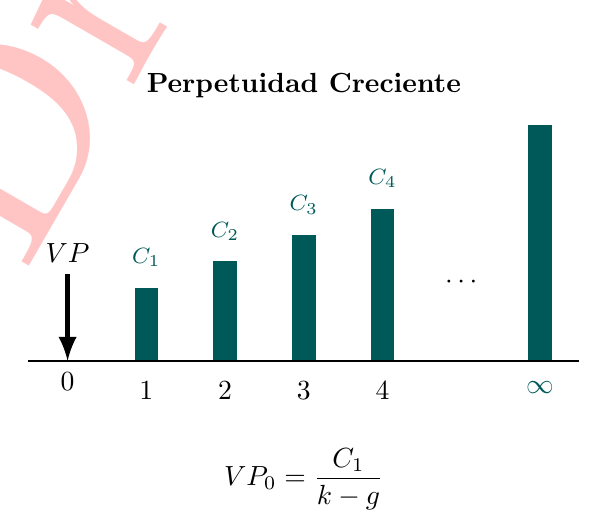
\begin{tikzpicture}
	\foreach \n in {1,...,4} 
	\draw [teal!70!black, line width = 3mm] 
	(\n,0) node [below] {\color{black}\(\n\)} 
	-- ++(0,0.6+\n/3) node [above] {\footnotesize \(C_\n\)};
	\draw [teal!70!black, line width = 3mm] 
	(6,0) node [below] {\(\infty\)} --++ (0,3);
	\node at (5,1) {\(\cdots\)};
	\draw [-latex, line width=0.7mm] 
	(0,1.1) node [above] {\(VP\)} -- (0,0) node [below] {\(0\)};
	\node at (3,3.5) {\textbf{Perpetuidad Creciente}};
	\node at (3,-1.5) {\(VP_0 = \dfrac{C_1}{k-g}\)};
	\draw (-0.5,0) -- (6.5,0);
\end{tikzpicture}

\end{document}


\espacio{4cm}
%=================Semblanza======================
\addcontentsline{toc}{section}{Semblanza y Análisis de Industria.}
\includepdf[pages=-,pagecommand={\thispagestyle{fancy}},height=\textheight]{../0.semblanza_eng/semblanza}


\chapter{DEVELOPMENT OF THE APPRAISAL.}\label{cap:5}
\thispagestyle{fancy}

%-----------------------Desarrollo del avalúo en la especie------------------------------------
\setcounter{section}{11}

\subsection{DEVELOPMENT OF THE VALUATION.}\label{sec:k2}

%\subsubsection{An\'alisis Financiero}


\subsubsection{An\'alisis Financiero}

Se recibieron los Estados financieros hist\'oricos del periodo de \EFde{}  a \EFhasta, por parte del  solicitante, seg\'un se muestran a continuaci\'on:

\begin{figure}[H]
\centering
\caption{Estados de Situaci\'on Financiera Hist\'oricos \EFdeHasta \label{fig:ESF}}\vspace{10pt}
\includegraphics[width=12cm]{../0.imagenes/EF_activo}\\[5pt]

\end{figure}

\begin{figure}[H]
\centering
\includegraphics[width=12cm]{../0.imagenes/EFpasivo_capital}\\

\end{figure}

\begin{figure}[H]
\centering
\caption{Estados de Resultados Hist\'oricos \EFdeHasta \label{fig:ESF}}\vspace{10pt}
\includegraphics[width=12cm]{../0.imagenes/ER}\\
\end{figure}


Para el an\'alisis financiero de dicha empresa, se llevaron a cabo los siguientes m\'etodos:
\begin{enumerate}
\item An\'alisis del Capital Invertido (IC\footnote{Investment Capital}).
\item Razones financieras de liquidez y solvencia (Ratios bancarios).
\item An\'alisis Dupont de 3 elementos.
\item An\'alisis de la Rentabilidad del Capital (ROC\footnote{Return on Capital}).
\item An\'alisis de la Rentabilidad del Capital Operativo Neto (ROIC\footnote{Return on Investment Capital}).
\end{enumerate}

\begin{figure}[H]
\centering

\underline{An\'alisis del Capital Invertido (IC)}\\[10pt]
\includegraphics[width=13cm]{../0.imagenes/IC}\\[10pt]

\underline{Razones financieras de liquidez y solvencia}\\[10pt]
\includegraphics[width=13cm]{../0.imagenes/ratios}\\[10pt]

\underline{An\'alisis Dupont}\\[10pt]
\includegraphics[width=13cm]{../0.imagenes/dupont}\\[10pt]

\underline{An\'alisis ROC}\\[10pt]
\includegraphics[width=13cm]{../0.imagenes/roc}\\[10pt]


\underline{An\'alisis ROIC}\\[10pt]
\includegraphics[width=13cm]{../0.imagenes/roic}\\[10pt]

\end{figure}





\subsubsection{Estimation of the Discount Rate Ke.}

The higher the systematic risk of a stock, the higher the return that investors will expect from equity securities. In order to estimate an appropriate discount rate in nominal terms and after taxes, the following inputs were used to determine the value of the \textcolor{principal}{Weighted Average Cost of Capital (WACC):}\\

\textcolor{principal}{Risk-free rate (Rf).} It is based on the yield of government bonds; in this case, the yield of the Mexican 10-year bond was considered, according to the website \url{Tradingeconomics.com}, with the following result:\\

\begin{figure}[H]
\centering
The risk-free rate obtained is \textbf{\rfValor\%}.\\[5pt]

\caption{Mexican  10-Year Bond Interest Rate Expectations}
 \includegraphics[width=9cm]{../0.imagenes_eng/rf}
\end{figure}


\gls{beta}. In order to determine the appropriate Beta ($\beta$) factor for the business, a market sample of levered betas from companies comparable to the valued business was considered:\\


\begin{figure}[H]
\centering
\includegraphics[width=.9\textwidth]{../0.imagenes_eng/beta_1}\\
\end{figure}

The levered beta of the sector corresponding to the company is \textcolor{principal}{\textbf{\valorBeta x}} (mean).\\

Unlevered Beta Formula:\\

\begin{figure}[H]
\centering
\includegraphics[width=8cm]{\rutaImagenes/beta_apalancada}
\end{figure}


The appraiser conducted the estimation of the unlevered BETA forecast for the business, having applied to the debt/equity ratio of the subject, the sample average, and the effective tax rate of the sector (ETR); with a result of \textcolor{principal}{\betaDesapalancada x}.\\

Relevered Beta Formula:\\

\begin{figure}[H]
\centering
\includegraphics[width=8cm]{\rutaImagenes/beta_reapalancada}
\end{figure}

Once the sector's unlevered BETA indicator was obtained, the appraiser carried out the estimation of the forecast for the relevered BETA to the business subject to valuation, having applied to the debt/equity ratio of the subject, the sector sample's median, and the Marginal tax rate of Mexico (MTR), with a result of  \textcolor{principal}{\betaReapalancada x}.\\

\textcolor{principal}{Equity Market Risk Premium:} It was obtained from the historical average of the difference in returns or ``spread'' between the Mexican stock market using the indicator known as the   enterprise risk premium (ERP).\\

\begin{figure}[H]
\centering
The enterprise risk premium is \textbf{\textcolor{principal}{\erpValor\%}} \\[10pt]

\includegraphics[width=.6\textwidth]{../0.imagenes_eng/erp}
\end{figure}

%\newpage
\textcolor{principal}{\textit{Size Prime}.} \\[5pt]

A size premium was applied to the firm, based on the book value of equity according to the following table.\\


\begin{figure}[H]
\centering
The Size Prime is \textbf{\textcolor{principal}{\sizePrime\%}} \\
\includegraphics[width=.5\textwidth]{\rutaImagenes/sp}
\end{figure}


Estimation of the Cost of Equity (Ke), resulting in \textcolor{principal}{\keValor\%}, 
in accordance with observable rates in the Mexican market:

\begin{figure}[H]
\centering
\includegraphics[width=10cm]{../0.imagenes_eng/ke}
\end{figure}









%\newcommand{\peersa}{Enterprise Value to total Revenues}
%\newcommand{\peersaTo}{Ingresos}
%\newcommand{\peersaMult}{1.18}
%\newcommand{\peersaEst}{Percentil 25}
%\newcommand{\peersb}{valor respecto de flujos de operativos del Sector (EV to EBITDA)}
%\newcommand{\peersbTo}{Ingresos}
%\newcommand{\peersbMult}{8.01}
%\newcommand{\peersbEst}{Percentil 25}
%\newcommand{\peersc}{Price to Book Value x}
%\newcommand{\peerscTo}{Ingresos}
%\newcommand{\peerscMult}{2.97}
%\newcommand{\peerscEst}{Mediana}
%\newcommand{\peersd}{Enterprise Value to EBIT}
%\newcommand{\peersdTo}{la Utilidad de Operaci\'on (EBIT):}
%\newcommand{\peersdMult}{19.16}
%\newcommand{\peersdEst}{Mediana}
%\newcommand{\peerse}{}
%\newcommand{\peerseTo}{la Utilidad de Operaci\'on antes de partidas virtuales e impuestos (EBITDA):}
%\newcommand{\peerseMult}{1.18}
%\newcommand{\peerseEst}{Percentil 25}
%
%\newcommand{\valorPeers}{}


\subsubsection{M\'ETODO DE VALUACI\'ON RELATIVA.}

\textcolor{principal}{Muestra de Mercado de Comparables de Cotizaci\'on (Trading Multiples o \gls{peers})}. Se aplic\'o el enfoque de mercado con base en un indicador conocido como ``\textcolor{principal}{\peersa} x''; con una estimaci\'on de \textcolor{principal}{\peersaMult x} \footnote{\peersaEst{} de la muestra} veces \peersaTo:\\



\begin{figure}[H]
\centering
\includegraphics[width=11cm]{../0.imagenes/peers_1}
\end{figure}

\newpage
Se aplic\'o el enfoque de mercado con base en un indicador conocido como ``\textcolor{principal}{\peersb} x''; con una estimaci\'on de \textcolor{principal}{\peersbMult x} \footnote{\peersbEst{} de la muestra} veces \peersbTo:\\

\begin{figure}[H]
\centering
\includegraphics[width=14cm]{../0.imagenes/peers_2}
\end{figure}

\newpage

Se aplic\'o el enfoque de mercado con base en un indicador conocido como ``\textcolor{principal}{\peersc} x''; con una estimaci\'on de \textcolor{principal}{\peerscMult x} \footnote{\peerscEst{} de la muestra} veces \peerscTo:\\

\begin{figure}[H]
\centering

\includegraphics[width=11cm]{../0.imagenes/peers_3}
\end{figure}

\newpage

Se aplic\'o el enfoque de mercado con base en un indicador conocido como ``\textcolor{principal}{\peersd} x''; con una estimaci\'on de \textcolor{principal}{\peersdMult x} \footnote{\peersdEst{} de la muestra} veces \peersdTo:\\

\begin{figure}[H]
\centering
\includegraphics[width=11cm]{../0.imagenes/peers_4}
\end{figure}

\newpage

Se aplic\'o el enfoque de mercado con base en un indicador conocido como ``\textcolor{principal}{\peerse} x''; con una estimaci\'on de \textcolor{principal}{\peerseMult x} \footnote{\peerseEst{} de la muestra} veces \peerseTo:\\

\begin{figure}[H]
\centering
\includegraphics[width=11cm]{../0.imagenes/peers_5}
\end{figure}



\subsection{Valor del negocio en marcha por PEERS.} El valuador llev\'o a cabo una capitalizaci\'on por m\'ultiplos para la estimaci\'on del valor razonable de la empresa, conforme al enfoque de mercado; seg\'un se aprecia: 

\begin{figure}[H]
\centering
\includegraphics[width=7cm]{../0.imagenes/valor_peers}\\

Valor razonable por PEERS: \textcolor{principal}{\$\valorPeers MXN}
\end{figure}
\subsection{APPLICATION OF THE DIRECT CAPITALIZATION METHOD. Through the income approach.} 


After conducting a detailed financial analysis of the business and given the difficulty in accurately projecting the revenues and cash flows of the entity due to its current negative equity and the variability of its historical figures, the appraiser decided to capitalize the NOPAT of the business with figures as of 2023, using a nominal capitalization rate that represents the opportunity cost of the business, along with the minimum expected appreciation of the Mexican economy, also taking into account the growth of such cash flows at a long-term inflation rate; having used the model of Geometrically Growing Annuity in accordance with the theoretical framework of corporate finance:\\


\begin{figure}[H]
\centering
\includegraphics[width=9cm]{../0.imagenes_eng/cap_dir}
\end{figure}



\newcommand{\ponda}{\peersa}
\newcommand{\pondaPorcentage}{10}
\newcommand{\pondb}{\peersb}
\newcommand{\pondbPorcentage}{20}
\newcommand{\pondc}{\peersc}
\newcommand{\pondcPorcentage}{10}
\newcommand{\pondd}{\peersd}
\newcommand{\ponddPorcentage}{30}
\newcommand{\ponde}{\peersd}
\newcommand{\pondePorcentage}{30}

\subsection{VALOR RAZONABLE PONDERADO DEL NEGOCIO EN MARCHA, CON CIFRAS AL \fechaValoresCorto.}

A continuaci\'on se concluye el valor razonable de la firma (\textit{\gls{firmvalue}}), a la fecha de valores, habi\'endose dado la siguiente importancia a los modelos en la ponderaci\'on: i) Un peso del \pondaPorcentage\% al modelo de valuaci\'on relativa conocido como \ponda{}, ii) Un peso del \pondbPorcentage\%  al modelo de valuaci\'on relativa (\gls{peers}) conocido como \pondb{} x; iii) Un peso del \pondcPorcentage\%  al modelo de valuaci\'on relativa (\gls{peers}) conocido como \pondc{} x; iv) Un peso del \ponddPorcentage\%  al modelo de valuaci\'on relativa (\gls{peers}) conocido como \pondd{} x;  v) Un peso del \pondePorcentage\%  al modelo de valuaci\'on relativa (\gls{peers}) conocido como \ponde{} x; seg\'un se muestra a continuaci\'on:

\begin{figure}[H]
\centering
\includegraphics[width=12cm]{../0.imagenes/valor_ponderado_firma}\\[10pt]

\textbf{\textcolor{principal}{Valor de la Firma al  \fechaValoresCorto:} \$\valorFirma{} \monedaCode}\\[5pt]
(\textcolor{principal}{\valorFirmaLetra{} \moneda{} 00/100 M.N.})
\end{figure}

%\newcommand{\valorCapitalM}{906}
%\newcommand{\valorCapitalm}{356}
%\newcommand{\valorCapitalc}{853}
%\newcommand{\valorCapital}{\valorCapitalM,\valorCapitalm,\valorCapitalc}
%\newcommand{\valorCapitalLetra}{\Numberstringnum{\valorCapitalM}{} millones, \numberstringnum{\valorCapitalm}{} mil, \numberstringnum{\valorCapitalc}}

\subsection{VALOR RAZONABLE DEL CAPITAL ACCIONARIO, CON CIFRAS AL \fechaValoresCorto}

A continuaci\'on se concluye el valor razonable del capital accionario (\textit{\gls{equityvalue}}), a la fecha de valores:\\

\begin{figure}[H]
\centering
\textbf{\textcolor{principal}{Valor del Capital Accionario al \fechaValoresCorto:} \$\valorCapital{} MXN}\\
\includegraphics[width=8cm]{../0.imagenes/valor_cap_acc}\\
(\textcolor{principal}{\valorCapitalLetra{} pesos 00/100 M.N.})


\end{figure}

\subsection{Fair Value per Share.}

At the express request of the applicant, the appraiser proceeded to calculate the fair value corresponding to each share. Therefore, the number of shares available was first accounted for (according to the information provided by the applicant), and then the total fair value of the Equity was divided by the number of shares; thus obtaining a  \textcolor{principal}{unit value per share of \$328.19 pesos per share}, as can be seen:

\begin{figure}[H]
\centering
\includegraphics[width=12cm]{../0.imagenes_eng/valor_por_accion}\\

\textbf{\textcolor{principal}{Conclusion:}}\\

\textbf{\$328.19 MXN}\\
(\textcolor{principal}{Three hundred twenty-eight pesos 19/100 M.N.})
\end{figure}

%-----------------------FECHA DE INSPECCIÓN---------------------
\section{INSPECTION DATE}\label{sec:l}
Not applicable.

%------------------------FECHA DE VALORES------------------------
\section{REFERENCE DATE FOR VALUE}\label{sec:m}
\fechaValores.

%-----------------------FECHA DEL INFORME-----------------------
\section{VALUATION REPORT DATE}\label{sec:n}
\fechaInforme.

%----------------------FUENTES DE INFORMACIÓN--------------
\section{SOURCES OF INFORMATION}\label{sec:nn}
\begin{itemize}

\item To obtain economic data for Mexico such as inflation, please consult the website of the National Institute of Statistics and Geography (INEGI): \url{http://www.inegi.org.mx/sistemas/IndicePrecios/}

\item For financial information related to industry, sector, discount rates, and peers, you can visit: \url{https://www.refinitiv.com/en}

\item To access reference data on risk-free rates for Mexico, please refer to the website of the Bank of Mexico: \url{www.banxico.org.mx}

\item For obtaining macroeconomic indicators, you can find information from ``Economía en breve'' by Mtro. Mario Correa at: \url{https://www.youtube.com/channel/UCtt93euOsTuq_gjUiZV-MSA}

\item For other financial data, you can visit the following websites:
\begin{itemize}
\item\url{www.damodaran.com}
\item \url{www.reuters.com}
\item \url{www.bmv.com.mx}
\item \url{www.sat.gob.mx}
\end{itemize}

\item For sector analysis, brand profiles, and the macro environment, you can access Passport Euromonitor at: \url{https://www.portal.euromonitor.com/}
\begin{itemize}
\item \url{https://www.vivo.com/en}
\item \url{https://www.vivo.com/mx}
\item \url{https://www.statista.com/statistics/541618/vivo-smartphone-shipments-worldwide/}
\item Vivo share of global smartphone shipments 2019-2023. Statista
\item Vivo Communication Technology. Crunchbase Company Profile \& Funding
\item La venta de ``smartphones'' mueve 93.000 millones hasta marzo: qué marcas suben y cuál se desploma? \url{elpais.com}
\end{itemize}
	 
\end{itemize}
%-----------------------CONSIDERACIONES PREVIAS A LA CONCLUSI\'ON------------------
\section{PRELIMINARY CONSIDERATIONS BEFORE CONCLUSION}\label{sec:o}
\begin{enumerate}


\item This study is only valid for the purpose and use specified in sections H and I of this report and when it is signed by the valuator.
\item The statements of facts, data, and documents provided by the requester for the preparation of this report are assumed to be true and correct.
\item  The analysis and opinions reported in this report are limited only by the assumptions and limiting conditions reported and are the result of the professional and impartial conclusions of the signing valuator.
\item  The signing valuator has no present or future interest in the conclusive figures that are the subject of this report, nor does the valuator have personal interests or bias with respect to the involved parties.
\item  The economic compensation of the valuator is not conditioned on the report of a predetermined or directed value that favors the requester's cause.
\item  This valuation report may only be used in its entirety and not in parts. No part of the report may be used in conjunction with any unrelated study. The publication of the report or any of its parts without the written authorization of the undersigned Public Broker is prohibited. This appraisal may not be used by any person or entity other than the one to which it is addressed or for a purpose or use other than stipulated.
\item  This study does not validate or indicate the legal, accounting, and/or tax treatment of the conclusive figures in the report in accordance with the financial information standards (NIF), the Income Tax Law, the VAT Law, and other applicable regulations.
	
\end{enumerate}

\chapter{CONCLUSIONS.}\label{cap:6}
\thispagestyle{fancy}
%-----------------------CONCLUSIÓN DE LA VALUACIÓN-----------------------
\setcounter{section}{16}
\section{VALUATION CONCLUSION.}\label{sec:p}
\textcolor{principal}{\underline{FIRST.-}}  The \textcolor{principal}{FAIR VALUE} of the company \textcolor{principal}{\empresaSolicitante}  as an ongoing business (\textit{\gls{firmvalue}}), as well as its \textit{\gls{equityvalue}} according to the application of the valuation models described in chapters \ref{cap:4} and \ref{cap:5} of this report, with a valuation date of \fechaValores, according to the purpose and use of the appraisal, is for the following amount:\\


\begin{center}
\textcolor{principal}{Firm Value as of \fechaValoresCorto:}\$\valorFirma{} MXN\\

(\textcolor{secundario}{\valorFirmaLetra{} pesos 00/100 M.N.})

\begin{figure}[H]
\centering
\includegraphics[width=12cm]{../0.imagenes_eng/valor_ponderado_firma}
\end{figure}


\textbf{\textcolor{principal}{Equity Capital Value as of \fechaValoresCorto:} \$\valorCapital{} MXN}\\
(\textbf{\textcolor{secundario}{\valorCapitalLetra{} pesos 00/100 M.N.}})\\
\end{center}

\begin{figure}[H]
\centering
 \includegraphics[width=7.5cm]{../0.imagenes_eng/valor_cap_acc}

\end{figure}
\espacio{.5cm}


\textcolor{principal}{\underline{SECOND.-}} The fair value per share as of \textcolor{principal}{\fechaValoresCorto}  is \$328.19 pesos per share, as detailed:
\begin{figure}[H]
\centering

\textcolor{principal}{Fair Value Per Share as of \fechaValoresCorto:} \textbf{\$328.19MXN}\\[5pt]
(\textcolor{secundario}{Three hundred twenty-eight pesos 19/100 M.N.})\\[10pt]

 \includegraphics[width=9cm]{../0.imagenes_eng/valor_acciones}

\end{figure}


\vspace{2cm}
To the best of my judgment and opinion, on the \textcolor{principal}{\diainforme th day of \monthname[\mesinforme]{}, \annoinforme{} (\numberstringnum{\annoinforme})}, according to the valuation criteria explained in the development of this report, I issue this VALUATION REPORT, with a VALUATION DATE as of \fechaValores; for all purposes as appropriate.\\



\begin{table}[H]
\centering
	\begin{tabular}{c}
	\begin{minipage}{7cm}
	\begin{center}
		``APPRAISER''\\[1cm]
		
		\rule{7cm}{.4pt}\\
		\nombrePerito\\
		\textcolor{principal}{Public Broker No. 2 of the State of Mexico, Specialist in business valuation, professional license number 10548258
		}
		
	\end{center}
	\end{minipage}
	
	\end{tabular}
\end{table}
%----------------------REPORTE FOTOGRAFICO------------------------------
\section{PHOTOGRAPHIC REPORT}\label{sec:q}
Not applicable.
%---------------------ANEXOS-------------------------------------------------------- 
\section{APPENDIX}\label{sec:r}

Appendix 1.- Corporate Information. Appendix 2.- Financial Information.



\label{lastpage}
\end{document}
